%One of the main goals in scientific research is coming up to quantum simulation; this is due to the fact that in several physical fields there are mechanisms that cannot be simulated by classical computers: the essential aim is using a controlled quantum device to investigate another quantum system. Experiments have shown that superconducting circuits are able to manipulate and measure at the level of a few qubits and microwave photons, as a quantum simulator~\cite{Nat.Phys2012}. They can be treated as open systems because of the loss of photons, coupled to the feeding in additional photons through continuous external driving. Moreover, they are greatly flexible, because of their nanofabricated nature and almost every parameter involved is widely tunable. In~\cite{PhysRevX.7.011016}, it has been demonstrated that QED cavity lattices act as a controllable platform guiding understanding of non-equilibrium physics. 

\chapter{Quantum Simulators of Open Many-Body Quantum Systems}
Open many-body quantum systems are difficult to study, due to the exponential growth of the number of freedom degrees with respect to the number of the constituent particles. The scientific community has built many strategies to overcome this obstacle, by developing and refining several analytical and numerical methods. In addition to these, another approach was proposed, based on the use of quantum simulators.

In the present chapter it is reported a review of some of the most relevant idea in the field of quantum simulators; in particular, the last section focuses on the simulation of spin systems, of remarkable interest in view of the model studied in this work.

%\section{Basics of Dynamics}
%As expressed in the previous chapter, an open quantum system can be described in terms of %$\rho_S$, the reduced matrix given by averaging over the environment: 
%\begin{equation}
%    \rho_S = \Tr_E(\rho).
%\end{equation}
%Under certain conditions discussed in section~\ref{appr_dynam_oqs}, the evolution of %$\rho_S$ is delineated by the Lindblad master equation:
%\begin{equation}
%\label{eqn:lindbladME_manyBody}
%    \dot{\rho_S} = -i[H_{sys}, \rho_S] - \sum_{a=1}^{N^2-1} %\gamma_a\mathcal{D}[L_a]\rho_S,
%\end{equation}
%where the first term expresses the usual unitary evolution under the system Hamiltonian %$H_sys$ and the second term represents the influence of the environment over the system %through the dissipation rate $\gamma_a$ and the dissipators
%\begin{equation*}
%    \mathcal{D}[L_a]\rho_S \equiv \frac{1}{2} \Bigl( [L_a\rho_S, L_a^{\dagger}] + [L_a, %\rho_S L_a^{\dagger}] \Bigl).
%\end{equation*}
%The Linblad operators determine the nature of the decoherence process, e.g. photon loss %($a$), qubit relaxation ($\sigma^-$), qubit dephasing ($\sigma^z$), and so on.
%The steady-state solution can be found rewriting this equation in terms of a linear %algebra problem. First of all, the Hilbert space for a system consisting of N spins, has %an orthonormal Fock-state basis such as $\ket{\phi_1, \phi_2, \dots \phi_N}$.
%For solving the equation
%\begin{equation*}
%    \dot{\rho}_S = 0,
%\end{equation*}
%outlining a \emph{superoperator formalism}~\cite{davRoss_wordpress} is advantageous. 
%Every linear operator $\hat{A}$ acting on the Hilbert space $\mathcal{H}$ can be associated with a vector in a superoperator space:
%\begin{equation*}
%    \hat{A} = \sum_{ij} A_{ij} \ket{i}\bra{j} \quad \rightarrow \quad |A\rangle\rangle = \sum_{ij} A_{ij} \ket{i}\ket{j}.
%\end{equation*}
%This way, the density operator can be vectorized and re-arranged as a \emph{super-ket} $|\rho_S\rangle\rangle$ with $N^2$ components, allowing eq.~\ref{eqn:lindbladME_manyBody} to be formally rewritten in terms of the Liouvillian superoperator. Thus, the steady-state equation can be read as an eigenvalue equation:
%\begin{equation}
%\label{eqn:SS_masterEq}
%    \hat{L}|\rho_S\rangle\rangle = 0.
%\end{equation}
%Its solution can be obtained computing the eigenvector of the $N^2 \times N^2$ super-operator $\hat{L}$ corresponding to the null eigenvalue.

%It is important to stress that the number of elements of the matricial representation of the superoperator grows with $N^4$. So, straightforward brute-force integration methods become unfeasible even for small system sizes.

\section{Quantum Simulators: Controllable Many-Body Systems}
In order to overcome the mentioned problem, over the years several analytical and numerical methods have been developed. In addition to these more "traditional" approaches, during the last years it arose the idea of studying a quantum system by using a properly designed quantum device. The essential aim of this new strategy lies in the employment of controlled quantum devices called \emph{quantum simulators}; they are systems able to experimentally emulate the Hamiltonian model bearing the non-trivial properties of the system under study. The usefulness of this approach is twofold~\cite{Tomadin_Fazio}:  not only it allows to explore properties of the model in regions that are elusive to the analytical and numerical studies, but also it consents to test to which limits the Hamiltonian model is appropriate to describe the system or whether additional ingredients are required.

Since the Josephson junction arrays~\cite{josephsonArrays}, that were probably the first quantum simulators in Physics History, much progress have been made especially with the advent of cold atoms in optical lattices.

\subsection{Cold Atoms in Optical Lattice}
\begin{figure}
    \centering
    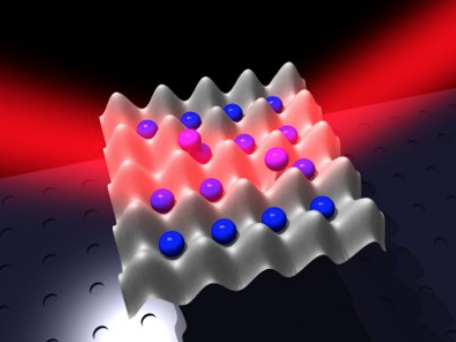
\includegraphics[scale=0.7]{Figures/optical_lattice.png}
    \caption{Optical lattices are crystals made of light: lasers beams interfere to form a periodic potential in which ultracold atoms are trapped. Figure taken from LENS website.}
    \label{fig:optical_lattice}
\end{figure}

The employment of cold atoms in optical lattices has proved to be a successful way to create simulators of a large variety of strongly interacting systems~\cite{ultracoldAtoms_condMatter}. 

In short, optical lattices are created by making laser beams counter-propagating interfere with each other~\cite{optical_lattice_interview}. The result is a standing wave with a periodic pattern (see sketch in fig.~\ref{fig:optical_lattice}). Then, ultracold atoms can be trapped in the potential wells, creating first a Bose-Einstein condensate or a cold gas of fermionic atoms and then slowly ramping up the laser beams to create the periodic lattice potential. 

Ultracold atoms in optical lattices represent nearly perfect realization of fermionic and bosonic Hubbard models\footnote{The (fermionic) Hubbard model in one dimension is characterized by the following Hamiltonian:
\begin{equation*}
    \mathcal{H} = -t\sum_{\langle ij \rangle}a^{\dagger}_{i\sigma}a_{j\sigma} + U\sum_i n_{i\uparrow}n_{i\downarrow},
\end{equation*}
where the first term represents the hopping between adjacent sites and the second represents the on-site interaction between particles. The $n_{i\sigma}$ are the occupation numbers, that count the number of electron with spin $\sigma$ in site $i$.
In the text, the plural \emph{Hubbard models} refers to the several variations of this model.
}~\cite{ultracoldAtoms_condMatter} and they are usually employed to simulate non-dissipative systems. However, new efforts have been made in order to introduce dissipation in these devices. 
In fig.~\ref{fig:optical_lattice_dissipation}, a sketch of the implementation of the effective dissipative process in an optical \emph{superlattice} is shown. The so-called superlattice is made up coupling driven-dissipative ultracold atoms in an optical lattice with a coherently driven reservoir. 

\begin{figure}
    \centering
    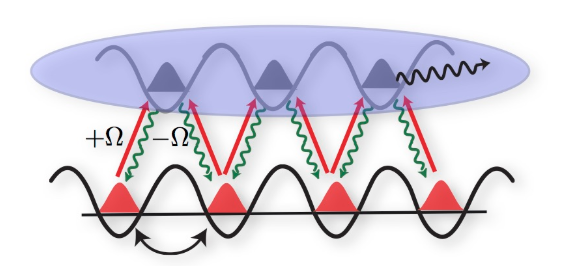
\includegraphics[scale=0.7]{Figures/optical_lattice_dissipation.png}
    \caption{Schematic realization of the effective dissipative process with ultracold atoms in an optical superlattice. Figure taken from~\cite{diehl_wEbsite}.}
    \label{fig:optical_lattice_dissipation}
\end{figure}

An interesting study over the possibility of using cold atoms to simulate dissipative many-body systems, has been done by~\cite{BEC_dissipativeMBsimulator}. In this work, they discuss the example of a driven dissipative Bose-Einstein condensate of bosons, where atoms in optical lattice are coupled to a bath of Bogoliubov excitations; the atomic current represents local dissipation. It was assumed that the atoms can be described by a Hubbard model, having the following Hamiltonian:
\begin{equation}
    \mathcal{H} = \mathcal{H}_0 + V \equiv -J \sum_{\langle i,j \rangle} a_i^{\dagger} a_j + \frac{1}{2}U \sum_i a_i^{\dagger 2} a_j^2,
\end{equation}
where $\mathcal{H}_0$ represents the kinetic energy of bosons hopping between
adjacent lattice sites with amplitude J, V is the onsite interaction
with strength U and $a_i$ ($a_i^{\dagger}$) are bosonic destruction (creation)
operators for atoms at i-th site. At this point, an appropriate choice of jump operators allows to couple the system to a bath so that it is driven to a pure many-body state by quasi-local dissipation. Applying standard linearization schemes in the weakly interacting situations led to obtain the solution of the master equation~\ref{eqn:SS_masterEq}. The steady-state solution seems to have properties similar to those of bosons in thermal contact to a heat bath.

Another strategy involves trapping Rydberg atoms in optical lattices. Rydberg atoms are alkali-like atoms with a single electron promoted into a highly excited orbital~\cite{carusotto_ciuti}. The presence of this atoms enhances photon-photon interaction; the presence of a single photon in the system is able to drive away from resonance condition all atoms contained in a surrounding volume. If the optical density is sufficiently high, a second photon travelling across this volume can be absorbed or suffer a phase shift; this can be use to obtain an effective blockade effect. \textcolor{red}{See ref. Lee Haffner Cross}

\subsection{QED-Cavity Arrays}
In the last few decades the field of quantum simulators has been enriched by a new idea, based on arrays of QED cavities~\cite{Tomadin_Fazio} (sketched in fig.~\ref{fig:QED_cavities}), in which light resonates and interacts with matter contained therein.  A compelling aspect of this kind of devices is the competition between two phenomena: while on the one hand light-matter interaction inside the cavity leads to photon blockade, on the other photon hopping between neighbouring cavities favors delocalization.

QED cavities are mathematically described by the Jaynes-Cummings model~\cite{shore_knight}, in which one mode of the cavity interacts with a two-level system. By ignoring light-matter interaction, a single cavity confines several modes of electromagnetic field and each of them is quantized as a harmonic oscillator. If one considers a cavity with a single mode with frequency $\omega$, the Hamiltonian describing such a system can be written as
\begin{equation}
\label{eqn:single_cavity}
    \mathcal{H} = \omega a^{\dagger}_la_l,
\end{equation}
where $a_l (a_l^{\dagger})$ annihilates (creates) a quantum of light in the mode of the l-th cavity.
An array of cavities sufficiently close to allow for photon hopping, can be described by eq.~\ref{eqn:single_cavity} to which the following term should be added:
\begin{equation*}
    \mathcal{H}_{hop} = -J (a^{\dagger}_la_l + h.c.),
\end{equation*}
where J is associated with the tunneling rate.
Now, if the light-matter interaction is introduced, the Hamiltonian can be written in this way:
\begin{equation}
    \mathcal{H} = \sum_l \mathcal{H}_l^{(0)} - J \sum_{\langle l, l' \rangle}(a^{\dagger}_la_l + h.c.),
\end{equation}
where the term $\mathcal{H}_l^{(0)}$ describes the light-matter interaction. In particular, we want to study QED cavities so the Hamiltonian term $\mathcal{H}_l^{(0)}$ is the Jaynes-Cummings model:
\begin{equation}
\label{eqn:Jaynes-Cummings}
    \mathcal{H}_{l,JC}^{(0)} = \varepsilon \sigma^z_l + \omega a^{\dagger}_la_l + g(\sigma^+_l a_l + \sigma^-_l a_l^{\dagger}),
\end{equation}
where $\sigma^\pm_l$ are the raising/lowering operators for the two-level system and $\varepsilon$ states the transition energy between the two levels.
The spectrum of the Hamiltonian~\ref{eqn:Jaynes-Cummings} is anharmonic, meaning the presence of the two-level system induces a repulsion between the photons in the cavity, so that in the cavity only a photon can be present at the same time. Qualitatively, this can be explained by the fact that a single photon in the cavity modifies the effective resonance frequency, so that the injection of another photon is inhibited. This nonlinear process is known as \emph{photon blockade} and has been named in analogy of the Coulomb blockade effect of electron transport through mesoscopic devices.
% QED cavities
    % sketch of QED cavities
    % optical cavities: photon blockade effect
    % Jaynes-Cummings nonlinearities
% pag. 55 Carusotto-Ciuti
% fig.10 di Noh2016

An array of cavities in the impenetrable photon regime has been theoretically studied~\cite{carusotto_ciuti}. As sketched in fig.~\ref{fig:cavities_ring}, a continuous pumping is considered. The transmission and/or absorption spectrum of the system shows the Tonks-Girardeau nature of the steady-state of photon gas, i.e. the fermionization of photons. \textcolor{red}{FINIRE DI SPIEGARE}

\begin{figure}
    \centering
    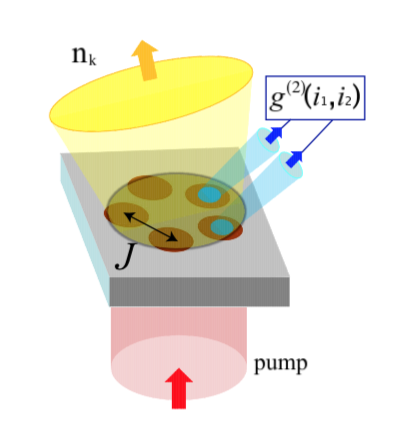
\includegraphics[scale=0.7]{Figures/cavities_ring.png}
    \caption{Sketch of an array of five cavities arranged in a ring geometry with periodic boundary conditions; the system is driven by a laser. Figure taken from~\cite{carusotto_ciuti}.}
    \label{fig:cavities_ring}
\end{figure}


\begin{figure}
    \centering
    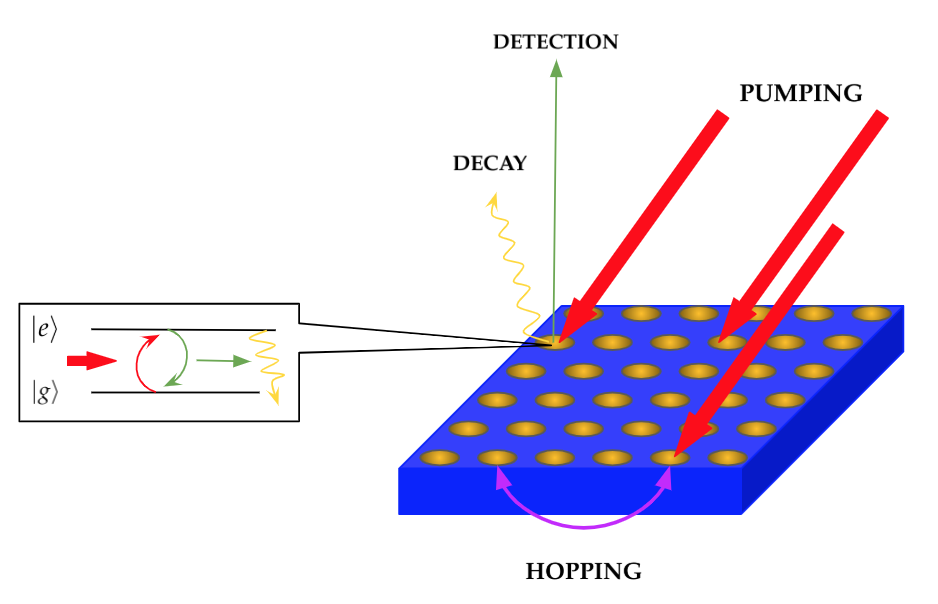
\includegraphics[scale=0.7]{Figures/QED_cavity.png}
    \caption{Sketch of array of QED cavities. In the inset there is a draft of the interaction between the two-level system and the photon resonating in the cavity and then decaying. Photons in the cavities have finite life-time, so there is a coherent external drive.}
    \label{fig:QED_cavities}
\end{figure}

% pag.5 Tomadin-Fazio per optical lattices vs cavity arrays

\subsection{Superconducting Circuits}
As for QED-cavities, also for superconducting circuits, or QED-circuits, light-matter interaction is central. In this simulators~\cite{supercircuitsQED}, the quantum "particles" are excitations, not physical particles subjected to conservation laws, so they naturally access non-equilibrium physics. Photonic mode can be realized with on-chip microwave resonators, typically Fabry-Perot kind of cavities. A qubit coupled to such a resonator can be described by the Jaynes-Cummings model:
\begin{equation}
    \mathcal{H}_{JC} = \omega_r a^{\dagger}a+ \varepsilon\sigma^+\sigma^- + g(a\sigma^+ + a^{\dagger}\sigma^-),
\end{equation}
where $\omega_r$ and $\varepsilon$ are the the photon and qubit excitation frequencies, and $a^{\dagger}$, a, $\sigma^+$ and $\sigma^-$ denote the corresponding raising and lowering operators. An example of these devices can be seen in fig.~\ref{fig:superconducting_circuits}.

\begin{figure}
    \centering
    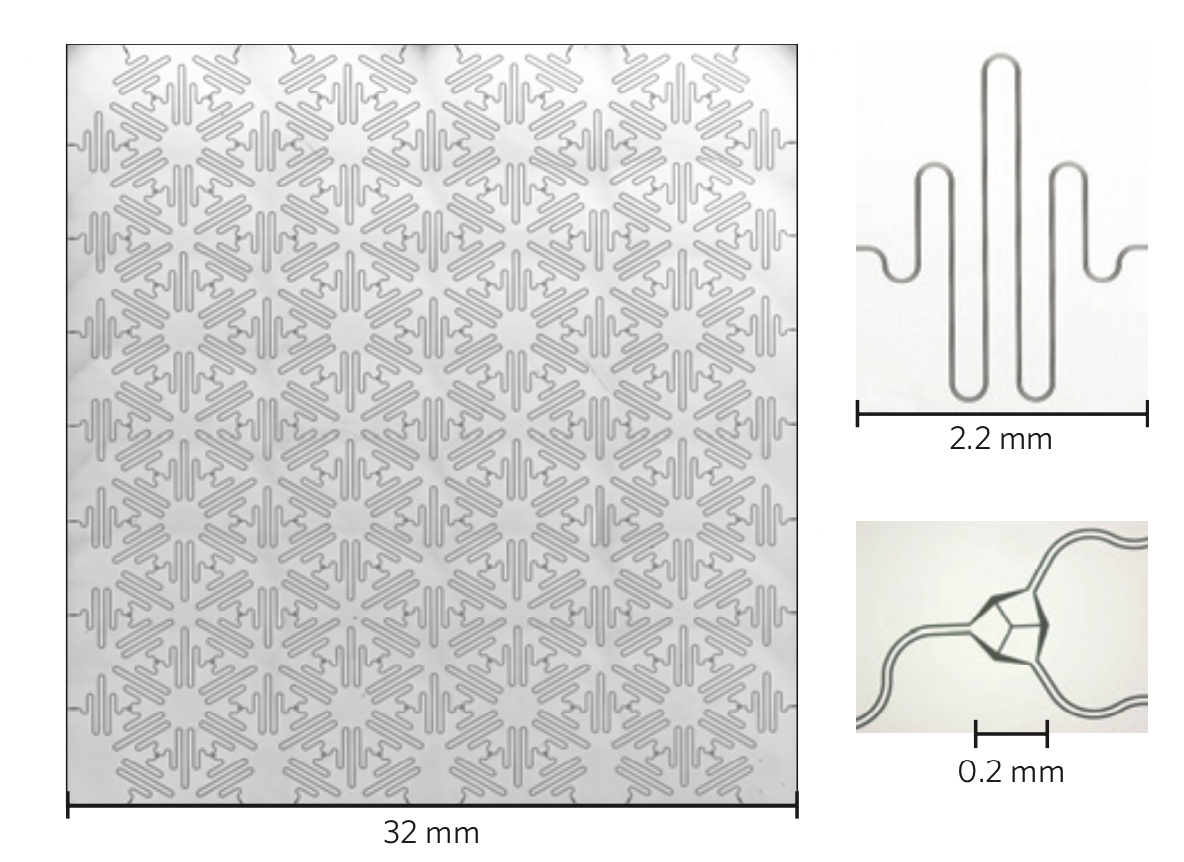
\includegraphics[scale=0.6]{Figures/superconducting_circuits.png}
    \caption{Example of an array of resonators forming a honeycomb pattern. On the left, more than two hundred microwave cavities are coupled in a Kagome lattice, a natural two-dimensional lattice. Each cavity is coupled to two neighbours, through a capacitor that enables photon hopping. On the bottom-right, it can be seen the simmetric three-way capacitor that ensures uniform hopping rates throughout the array. Figure taken from~\cite{supercircuitsQED}.}
    \label{fig:superconducting_circuits}
\end{figure}

\subsection{Arrays of Optomechanical Systems}
A recent proposal by~\cite{optomechanical_arrays} considers making arrays of optomechanical systems. The essential idea is that at each site of such an array, a localized mechanical mode interacts with an optical mode of a cavity driven by laser beams; the interaction occurs via radiation pressure. This way, both photons and phonons can hop between neighbouring sites. Because of the experimental complexity of this kind of device, only a single cavity has been cooled to the ground state~\cite{Lee_Haffner_Cross}, so far. 

The work of~\cite{optomechanical_arrays} focuses on the transition of the collective mechanical motion from an incoherent state (due to quantum noise) to an ordered state with phase-coherent mechanical oscillations; for this dynamics, the dissipative effects induced by the optical modes play a crucial role. Indeed, they allow the mechanical modes to have self-induced oscillations, once the optomechanical amplification rate exceeds the intrinsic mechanical damping; on the other hand, the quantum noise prevents the mechanical modes to synchronizing.


\section{Quantum Simulation of Spin Systems}
Interacting two level systems, either spins or qubits, are of central importance in Quantum Information and Condensed Matter Physics. 
%\textcolor{red}{In magnetic compounds where spin lattices appear naturally the addressability of individual spins is unfortunately extremely hard to achieve because the spatial separation between neighboring spins is very small and the timescales of interesting processes can be very short.}

Since the discover of the \emph{photon blockade}~\cite{ph_blockade} arose the fact that the cavity mode is well described by a spin-$1/2$ Hamiltonian. Few years later, the Jaynes-Cummings model in the Mott regime was shown to simulate a XY spin model~\cite{angelakis}. In particular, the studied system consisted of coupled electromagnetic cavities doped with single two-level system; it is shown the possibility of observing an insulator phase of total (atomic plus photonic, i.e. \emph{polaritonic}) excitations. From such a system, an effective XY Hamiltonian arises, with spin up (down) corresponding to the presence (absence) of a polariton.

A scheme for realizing the Ising spin-spin interaction has been proposed in~\cite{LiGuGong}, where a system consisting in trapped two-level atoms in a one dimensional coupled microcavities. 

A more complicated system has been investigated in~\cite{Hartmann_XYZ}, which uses three-level atoms in micro-cavities coupled to each other via the exchange of virtual photons; it is shown that it can model an anisotropic Heisenberg spin-1/2 chain in an external magnetic field. The two spin polarizations $\ket{\uparrow}$ and $\ket{\downarrow}$ are represented by two long-lived atomic levels of a $\Lambda$ level-structure; let us see why. The quantized mode of the cavity together with external lasers can induce Raman transition between these two lowest-lying states.  With appropriately chosen detunings, the dominant Raman transition between the two lowest-lying states involves one laser and one cavity photon. This implies that the emission and absorption of virtual photons in the cavity is confined to only two states per atom, the long-lived ones, so that can be described by a spin-1/2 Hamiltonian. The coupling of virtual photons between neighbouring cavities simulates $\sigma^x\sigma^x$ and $\sigma^y\sigma^y$ interactions; the effective spin can be coupled to an effective magnetic field $\sigma^z$; using the same atomic level configuration but a different set-up of the external sources an effective $\sigma^z\sigma^z$ interaction is obtained.

\begin{figure}[H]
    \centering
    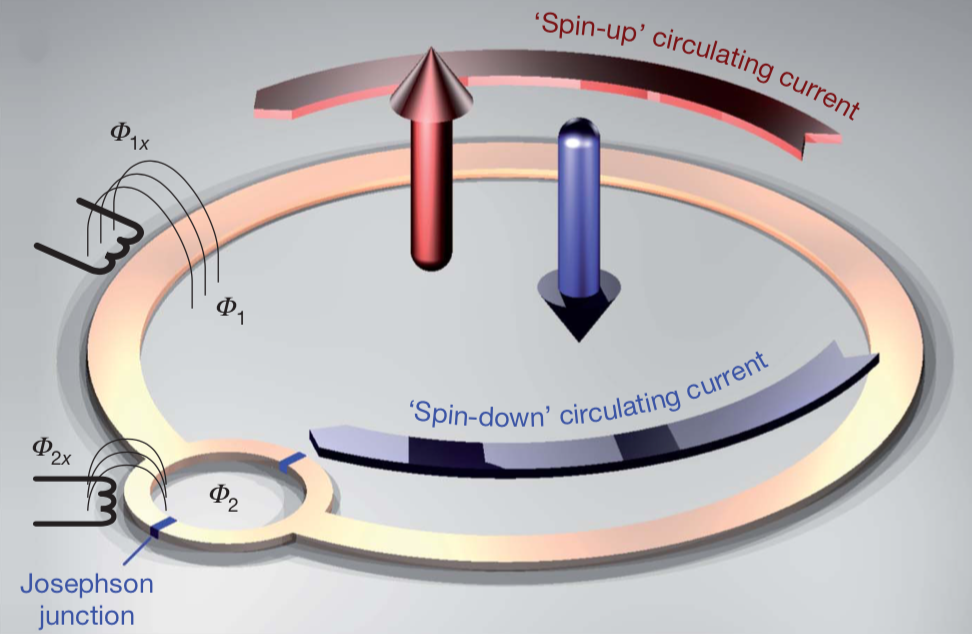
\includegraphics[scale=0.5]{Figures/superconductinCircuit_SpinSystem.png}
    \caption{Simplified schematic of a superconducting flux qubit \\acting as a quantum mechanical spin~\cite{8spinChain_simulatedByQubits}.}
    \label{fig:superconductinCircuit_SpinSystem}
\end{figure}

It has been possible using superconducting circuits to simulate small spin chains, by directly coupling a number of superconducting qubits~\cite{8spinChain_simulatedByQubits}. Fig.\ref{fig:superconductinCircuit_SpinSystem} shows two superconducting loops in the qubit, each subject to an external flux bias $\Phi_{1x}$ and $\Phi_{2x}$. The dynamics of the device can be modelled as a quantum mechanical double-well potential. The two lowest energy states of the system correspond to clockwise or anticlockwise circulating current in loop 1. Considering only these two states (in the limit of low temperature it is a valid approximation), the qubit dynamics is that of an Ising spin. Qubits are then coupled together using programmable coupling elements; this allows to tune the spin coupling in a continous way between ferromagnetic and antiferromagnetic. The behaviour of this system is well described by an Ising model Hamiltonian:
\begin{equation*}
    \mathcal{H} = \sum_{i=1}^{N} h_i\sigma_i^z + \sum_{i,j=1}^{N} J_{ij}\sigma_i^z\sigma_j^z.
\end{equation*}
In this way, it has been possible to simulate a one-dimensional 8-sites spin chain, with the ends polarized in opposite directions.